%% IEEE InGARSS 2026 -- 5-page conference manuscript (incl. references)
%% Build:  cd paper && pdflatex main && pdflatex main
%% Every number here traces to ../RESULTS_LOG.md ; every DOI verified via Crossref (2026-06-19).
\documentclass[conference]{IEEEtran}
\IEEEoverridecommandlockouts

\usepackage{cite}
\usepackage{amsmath,amssymb,amsfonts}
\usepackage{graphicx}
\usepackage{booktabs}
\usepackage{array}
\usepackage{xcolor}
\usepackage{url}

% Visible, non-fabricated placeholders for items still to be confirmed by the author (CLAUDE.md Rule 3).
\newcommand{\todo}[1]{\textbf{\textcolor{red}{[#1]}}}

\graphicspath{{figs/}}

\begin{document}

\title{Calibrated Probabilistic Early Warning of\\
Drought--Flood Abrupt Alternation over Bangladesh\\
from Satellite Earth Observation}

\author{\IEEEauthorblockN{Bishwadip Maitra}
\IEEEauthorblockA{Bangladesh University of Engineering and Technology (BUET)\\
Dhaka, Bangladesh\\
\todo{department / corresponding e-mail}}}

\maketitle

\begin{abstract}
The Bangladeshi monsoon can turn a district from drought to flood, or back, within a single season,
and the most damaging form of this variability is the swing itself rather than either extreme alone.
Operational systems nonetheless treat drought and flood separately and issue point forecasts that say
nothing about confidence. We present what is, to our knowledge, the first early-warning study of
drought--flood abrupt alternation (DFAA) for Bangladesh, built entirely from a satellite-derived
monthly record of thirteen stations spanning 2000--2022. We define a multivariate DFAA index from
rainfall, soil-moisture and SPEI anomalies, forecast its full predictive distribution one to three
months ahead with a monotone quantile model, and calibrate that distribution with conformalized
quantile regression so that the stated event probabilities mean what they say. The calibrated model
improves on a climatological reference at every lead (CRPS skill up to $+0.16$) and matches a physical
water-balance benchmark at detecting alternations (ROC-AUC up to $0.82$). Conformal calibration
restores the coverage the raw model loses, and the skill transfers to every held-out station. A
cost--loss analysis shows the probabilities carry decision value across a broad range of users. We also
document that the alternations have intensified since 2018, which both motivates the system and bounds
it.
\end{abstract}

\begin{IEEEkeywords}
Drought--flood abrupt alternation, probabilistic forecasting, conformal prediction, calibration, early
warning, climate adaptation, Earth observation, Bangladesh.
\end{IEEEkeywords}

\section{Introduction}
A Bangladeshi farmer can lose a crop to drought and then lose the replanting to a flood, both inside one
monsoon. The two disasters are usually studied, forecast, and insured against as though they were
independent, yet their most punishing form is the rapid handover from one to the other: parched soil
seals over, the next heavy spell runs off instead of soaking in, and a rain-fed system is left with
neither the storage to buffer a flood nor the moisture to survive the dry spell that may follow. This is
a compound event in the sense of Zscheischler \emph{et al.}~\cite{zscheischler2018}, and in monsoon Asia
it has a name---drought--flood abrupt alternation (DFAA). It is precisely the regime an early-warning
system built for a single hazard cannot see.

DFAA has a decade of study behind it, almost all of it over China. Wu and Li introduced a long-cycle
alternation index from large-scale atmospheric singularities over the Yangtze~\cite{wu2006}; later work
generalised it to a multivariate, multiscale form that folds in evapotranspiration and soil
moisture~\cite{bai2024}, and a recent review catalogues the mechanisms and the asymmetry between
drought-to-flood and flood-to-drought transitions~\cite{bai2023}. Bangladesh, despite sitting at the
sharp end of monsoon variability, has no DFAA study at all. What it does have is a growing
machine-learning literature for drought---seasonal prediction from weather
variables~\cite{mamun2024}, ensemble models for agricultural drought in the Ganges
delta~\cite{mondol2025}, SPI/SPEI forecasting in the northwest~\cite{akter2023}---and these share two
blind spots. They forecast a point value, and they forecast one hazard. The officer deciding whether to
pre-position pumps or draw down a reservoir needs neither a single number nor a drought-only outlook;
they need the probability of an abrupt swing, and they need that probability to be honest.

We close that gap. From a satellite-derived monthly record of thirteen stations across Bangladesh we
build the country's first DFAA index and event climatology, forecast the full predictive distribution of
the index one to three months ahead, and---the part missing from the regional literature---calibrate it
so that a stated 90\% interval covers the outcome 90\% of the time. Four findings follow. Alternations
have grown more frequent since 2018, which is both the reason to build the system and the reason it is
hard. A gradient-boosted quantile model beats climatology at every lead and keeps pace with a physical
water-balance benchmark at detecting events, earning the learning its place over both statistics and
physics. Conformal calibration recovers the coverage the raw model loses, and the skill transfers to
every held-out station. One honest negative runs throughout: the physics-guided features we engineered do
not help, and we say so.

\begin{figure}[t]
\centering
\fbox{\begin{minipage}[c][2.3cm][c]{0.93\columnwidth}\centering
\todo{Insert STUDY-AREA MAP (half column): the 13 BMD stations over Bangladesh, with relief/river network.}
\end{minipage}}
\caption{Study area: the thirteen Bangladesh Meteorological Department stations whose satellite-derived
monthly records (2000--2022) underpin this study.}
\label{fig:study}
\end{figure}

\section{Data and the DFAA Index}
Our record covers thirteen Bangladesh Meteorological Department stations at monthly resolution from
January 2000 to December 2022, 276 months each (Fig.~\ref{fig:study}). Every variable---rainfall, soil
moisture, the three-month Standardized Precipitation Evapotranspiration Index (SPEI)~\cite{vicente2010}, and daily
maximum and minimum temperature---is an Earth-observation product sampled at the station locations, which is what
places the work in the satellite remote-sensing domain rather than the rain-gauge one.
\todo{Confirm and cite the specific EO/reanalysis product and native resolution per variable (Rule 3).}
After dropping a single trailing all-missing row we retain $3{,}587$ clean station-months; one value
(Khulna, February 2018) is missing, and we flag rather than fill it.

We strip the seasonal cycle station by station. Rainfall and soil moisture are standardised against a
climatology fitted on the training years alone,
\begin{equation}
z_v(s,t)=\frac{x_v(s,t)-\mu_v\!\left(s,m(t)\right)}{\sigma_v\!\left(s,m(t)\right)},
\label{eq:z}
\end{equation}
while SPEI is kept as supplied, since it is already standardised. Monsoon soil moisture saturates at
field capacity, so a few station-months carry almost no historical variance; left unguarded,
\eqref{eq:z} divides by near-zero and diverges. We floor each monthly standard deviation at $0.15$ of
the station's pooled value and clip the anomaly at $\pm4$, both fitted on training data and applied
unchanged elsewhere. A single wetness state then combines the three moisture signals with equal weight,
$W=\tfrac{1}{3}\left(z_P+z_{SM}+\mathrm{SPEI}\right)$, signed so that positive means wet.

To turn the wetness trajectory into an alternation signal we adapt the long-cycle index of Wu and
Li~\cite{wu2006} to a monthly, multivariate form. Let $W_E$ be the mean wetness over the $h$ months
ending at the forecast origin $t$---the recent, observed state---and $W_L$ the mean over the $h$ months
that follow, the future we predict. The DFAA index is
\begin{equation}
\mathrm{DFAA}(s,t)=\left(W_L-W_E\right)\left(|W_E|+|W_L|\right)\,\alpha^{-|W_E+W_L|},
\label{eq:dfaa}
\end{equation}
with $\alpha=1.8$. Each factor earns its place. The first sets the direction and size of the swing:
positive for a drought-to-flood flip (DTF), negative for flood-to-drought (FTD). The second insists that
both windows be genuinely anomalous, so that noise around zero cannot pose as a swing. The third damps
persistent same-sign spells---a wet season after a wet season is not an alternation. We label a
station-month an event when $|\mathrm{DFAA}|$ exceeds $\theta_D$, the 80th percentile of
$|\mathrm{DFAA}|$ over the training years.

Fixing $\theta_D$ on the training period sets the training event rate to 20\% by construction. The test
years 2018--2022 carry 33\% (Fig.~\ref{fig:mech}). Read plainly, abrupt alternations have become half
again as common in the most recent stretch of the record. This is the finding that motivates the warning
system, and it is also what makes the forecast hard: the test distribution is heavier-tailed than
anything the model trains on, so any forecaster anchored to the past climatology is steering by a map
that the ground no longer matches.

\begin{figure*}[t]
\centering
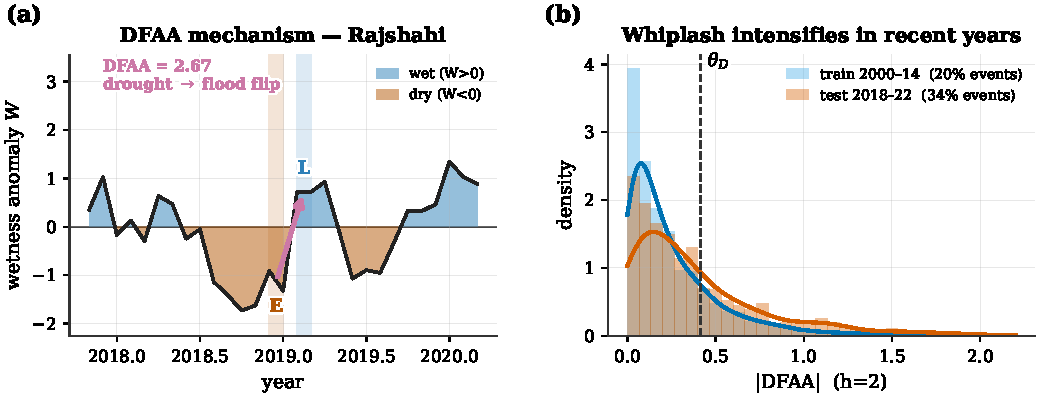
\includegraphics[width=\textwidth]{fig1_mechanism_intensification}
\caption{The mechanism and its trend. (a)~A representative drought-to-flood reversal: wetness $W$ swings
from a dry early window (E) to a wet late window (L), the configuration that \eqref{eq:dfaa} scores as a
large positive DFAA. (b)~Abrupt alternations are heavier-tailed in 2018--2022 than in 2000--2014; with
the event threshold $\theta_D$ fixed on the training years, the recent event rate climbs from 20\% to
33\%.}
\label{fig:mech}
\end{figure*}

\section{Method}
\textbf{Forecasting features.} Alongside the raw anomalies we compute a set of physics-guided
predictors: potential evapotranspiration by the temperature-based Hargreaves method~\cite{hargreaves1985},
\begin{equation}
\mathrm{PET}=0.0023\,R_a\,(\bar{T}+17.8)\sqrt{T_x-T_n},\quad \bar{T}=\tfrac{T_x+T_n}{2},
\label{eq:pet}
\end{equation}
the climatic water balance $D=P-\mathrm{PET}$, an antecedent precipitation index, soil-moisture and SPEI
tendencies, rolling three- and six-month totals, and calendar and location encodings. The same physics
motivates a baseline that needs no learning: a single-bucket water store that fills with rainfall,
empties with PET and spills when full, rolled forward $h$ months on climatological forcing and read out
through \eqref{eq:dfaa}. This bucket is the bar a learned model must clear to claim it has added anything
over hydrology.

\textbf{Predictive distribution.} We forecast the index as a set of quantiles rather than a single
value. To keep the quantiles ordered---a 90th percentile below the 10th is not a distribution---we use
the monotone composite head of Cannon~\cite{cannon2018}, which builds each quantile from the one below it
by adding a non-negative increment,
\begin{equation}
Q_{\tau_1}=b(\mathbf{x}),\qquad
Q_{\tau_k}=Q_{\tau_1}+\sum_{j=2}^{k}\mathrm{softplus}\!\left(\delta_j(\mathbf{x})\right),
\label{eq:head}
\end{equation}
trained with the pinball loss~\cite{koenker1978} averaged over the quantile grid, leads and samples,
\begin{equation}
\rho_\tau(u)=\max\!\left(\tau u,(\tau-1)u\right),\qquad u=y-Q_\tau .
\label{eq:pinball}
\end{equation}
Two learners share this target: gradient-boosted quantile regression (GBQ), in the spirit of
probabilistic boosting~\cite{duan2020}, and a compact recurrent network (QR-LSTM) carrying the same head
over a twelve-month window. We deliberately keep physics out of the loss---this is not a
physics-informed neural network~\cite{raissi2019}---because a record of $\sim\!3{,}600$ rows cannot
constrain a hard residual, and we avoid heavier sequence models (temporal fusion transformers, deep
rainfall--runoff LSTMs) for the same reason.

\textbf{Calibration.} A sharp forecast is worthless if its intervals are wrong, and the recent-period
shift gives every reason to expect they will be. We wrap the model in conformalized quantile regression
(CQR)~\cite{romano2019}, which measures on a held-out calibration set how far reality falls outside each
predicted interval and then widens the interval by exactly that much. For a central interval
$[Q_{\mathrm{lo}},Q_{\mathrm{hi}}]$,
\begin{equation}
E_i=\max\!\big(Q_{\mathrm{lo}}(\mathbf{x}_i)-y_i,\;y_i-Q_{\mathrm{hi}}(\mathbf{x}_i)\big),\;\;
\big[\,Q_{\mathrm{lo}}-\hat{E},\;Q_{\mathrm{hi}}+\hat{E}\,\big],
\label{eq:cqr}
\end{equation}
where $\hat{E}$ is the $\lceil(n{+}1)(1{-}\alpha)\rceil/n$ empirical quantile of $\{E_i\}$. The guarantee
is distribution-free and holds per lead. We calibrate on 2015--2017, strictly between the 2000--2014
training years and the 2018--2022 test years. The operational warnings come straight from the calibrated
predictive CDF $\hat{F}$:
\begin{equation}
P(\mathrm{DTF})=1-\hat{F}(+\theta_D),\qquad P(\mathrm{FTD})=\hat{F}(-\theta_D).
\label{eq:event}
\end{equation}

\textbf{Evaluation and leakage control.} We score the distribution with the continuous ranked
probability score (CRPS) and report skill over climatology as $\mathrm{CRPSS}=1-\mathrm{CRPS}/
\mathrm{CRPS}_{\mathrm{clim}}$~\cite{gneiting2007}; coverage with the prediction-interval coverage
probability (PICP) and the expected calibration error (ECE); event detection with ROC-AUC for DTF and
FTD; and operational value with a cost--loss analysis. Every climatology, scaler, threshold and
conformal radius is fitted on the training (or calibration) split alone and applied unchanged
downstream. Splits are time-ordered, and the transfer test leaves whole stations out; we never shuffle
the autocorrelated rows.

\section{Results}
\textbf{Beating climatology, matching physics.} Table~\ref{tab:main} gives the test-period scores. The
water-balance bucket is a capable detector---its DTF discrimination climbs from $0.65$ at one month to
$0.79$ at three---yet mediocre on the full distribution, and plain persistence is actively harmful,
because an alternation index reverts by construction. GBQ is the clear winner: it beats the
climatological reference on CRPS at every lead, and the margin \emph{widens} with lead, from $+0.094$ to
$+0.162$. This is not the model sharpening with distance but the reference collapsing faster---climatology
has no answer to the post-2018 shift, while a conditional model that reads the current state still does.
GBQ also matches or edges the physical bucket on event AUC (up to $0.82$) while delivering the calibrated
distribution the bucket cannot. The QR-LSTM trails at every lead; with only $\sim\!2{,}200$ training
origins, boosting uses the data better, and we keep it as an honest deep-learning reference.

\begin{table}[t]
\centering
\caption{Test-period (2018--2022) skill and calibration by lead $h$. CRPSS is relative to climatology
(skill $0$); higher is better. GBQ leads on CRPSS at every horizon, and conformal calibration (CQR)
restores the coverage the raw model loses while roughly halving the calibration error (ECE).}
\label{tab:main}
\small
\begin{tabular}{lccc}
\toprule
 & \multicolumn{3}{c}{lead $h$ (months)}\\
\cmidrule(lr){2-4}
metric / method & 1 & 2 & 3\\
\midrule
CRPSS, water-balance bucket & $-0.287$ & $-0.130$ & $+0.072$\\
CRPSS, QR-LSTM            & $+0.002$ & $+0.056$ & $+0.109$\\
CRPSS, \textbf{GBQ}      & $\mathbf{+0.094}$ & $\mathbf{+0.122}$ & $\mathbf{+0.162}$\\
\midrule
DTF-AUC, GBQ & $0.670$ & $0.745$ & $0.819$\\
FTD-AUC, GBQ & $0.780$ & $0.769$ & $0.746$\\
\midrule
PICP$_{90}$, GBQ raw      & $0.791$ & $0.707$ & $0.596$\\
PICP$_{90}$, \textbf{GBQ$+$CQR} & $\mathbf{0.928}$ & $\mathbf{0.863}$ & $\mathbf{0.844}$\\
ECE, GBQ raw\,$\to$\,CQR & $.036\,{\to}\,.024$ & $.072\,{\to}\,.040$ & $.106\,{\to}\,.063$\\
\bottomrule
\end{tabular}
\end{table}

\iffalse  % fig:skill disabled to meet the 5-page limit (its CRPSS/AUC values are in Table I). Re-enable if space allows.
\begin{figure*}[t]
\centering
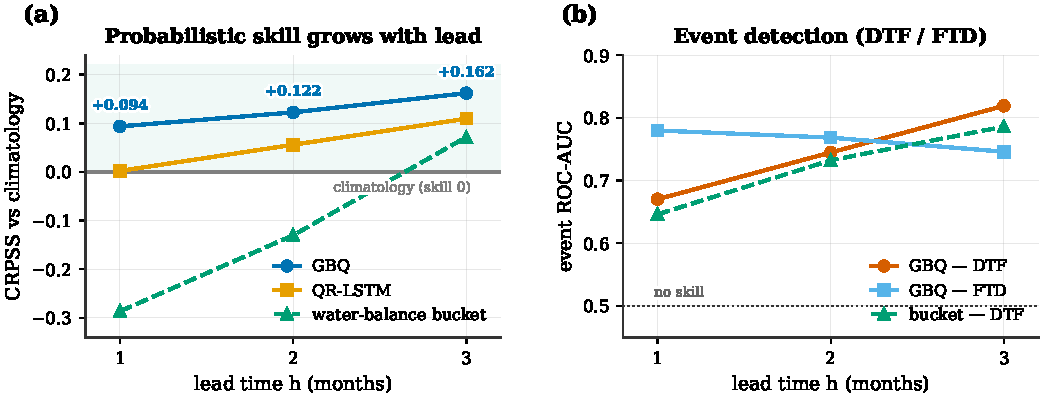
\includegraphics[width=\textwidth]{fig3_skill_leadtime}
\caption{Probabilistic skill and event detection on the test period. (a)~CRPS skill over climatology
rises with lead for GBQ because the climatological reference degrades under the recent-period shift, not
because the forecasts improve; persistence and the physics bucket lag behind. (b)~GBQ matches or edges
the water-balance bucket at detecting drought-to-flood (DTF) and flood-to-drought (FTD) events.}
\label{fig:skill}
\end{figure*}
\fi

\textbf{Making the probabilities honest.} The raw models are overconfident, and worse so at longer lead:
GBQ's nominal 90\% interval covers only 79\%, 71\% and 60\% of test outcomes at one, two and three
months. Conformal calibration repairs most of this, lifting coverage to 93\%, 86\% and 84\% and roughly
halving the calibration error at every lead (Fig.~\ref{fig:calib}; Table~\ref{tab:main}). What it cannot
fully repair is itself informative. At two and three months the calibrated coverage still sits a few
points below nominal, because conformal prediction assumes calibration and test data are exchangeable
and the 2018--2022 trend breaks exactly that: the radius learned on 2015--2017 is a touch too small for a
test period that has drifted further. We read the residual gap not as a failure of the method but as a
measurement of the non-stationarity itself.

\begin{figure*}[t]
\centering
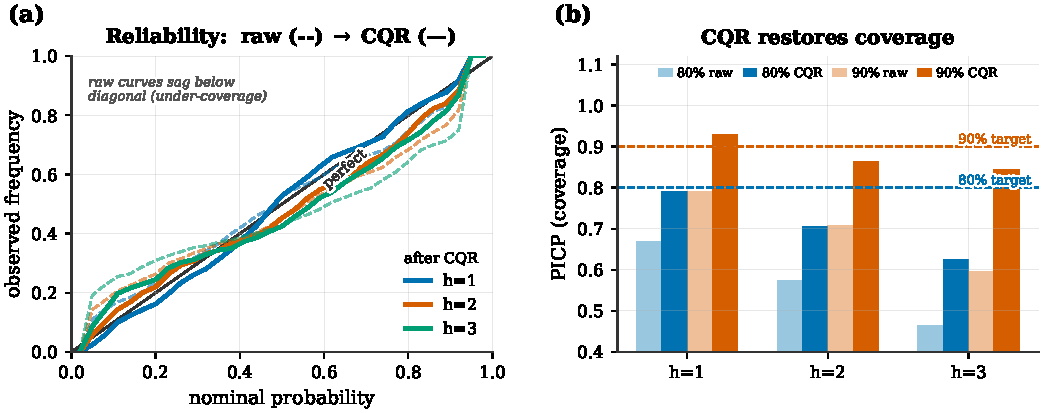
\includegraphics[width=\textwidth]{fig4_calibration}
\caption{Calibration. (a)~Reliability curves: the raw forecasts (dashed) sag below the diagonal, i.e.\
overconfident, and conformal calibration (solid) pulls them onto it. (b)~The nominal 80\% and 90\%
intervals recover most of their lost coverage after CQR; the small residual gap at $h=2,3$ is the
non-stationarity the method cannot absorb.}
\label{fig:calib}
\end{figure*}

\textbf{What the model uses, and what it does not.} Permutation importance is blunt about where the
skill comes from: the observed current wetness $W_E$ dominates every other input by more than an order of
magnitude, with seasonality and the soil-moisture anomaly a distant second. This
is honest to flag---because the index contains $W_E$ by construction and $W_E$ is observed at the
origin, part of the skill is current state plus mean reversion rather than genuine anticipation of the
future window. The physics-guided features add essentially nothing: dropping all of them shifts CRPSS by
$+0.001$, $-0.008$ and $-0.013$ across the three leads, within noise. Boosting on the raw anomalies
already extracts the moisture signal, and the hand-built PET and water-balance predictors are redundant
to it. We had hoped otherwise; we report the neutrality plainly, and it leaves the headline untouched,
since physics was scoped here as an ablation rather than a load-bearing part of the claim. The calibrated
probabilities do carry operational value: in a cost--loss framework the forecast is worth up to $0.37$
(DTF) and $0.41$ (FTD) of the climatology-to-perfect range at two months, and stays positive across
cost/loss ratios from roughly $0.06$ to $0.7$, so users from cheap-precaution to expensive-action would
act on it profitably.

\iffalse  % fig:drivers disabled to meet the 5-page limit; its content (W_E dominance, neutral physics ablation, cost--loss values) is in the prose. Re-enable if space allows.
\begin{figure*}[t]
\centering
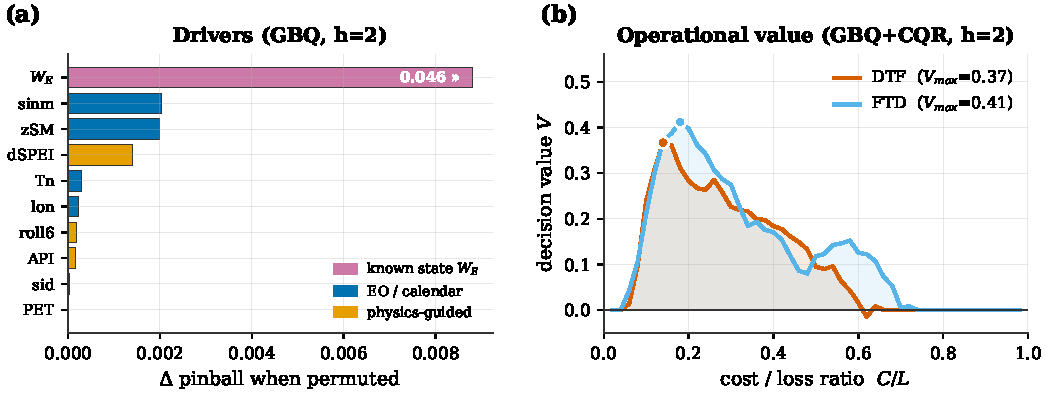
\includegraphics[width=\textwidth]{fig5_drivers_costloss}
\caption{Drivers and decision value. (a)~Permutation importance is dominated by the observed current
wetness $W_E$; the engineered physics-guided features (green) contribute within noise. (b)~In a
cost--loss framework the calibrated forecast carries positive value across a wide band of user cost/loss
ratios, peaking near $0.37$ (DTF) and $0.41$ (FTD) at two months.}
\label{fig:drivers}
\end{figure*}
\fi

\textbf{Where alternations strike, and whether the model travels.} The event climatology is uneven
(Fig.~\ref{fig:gis}; Table~\ref{tab:spatial}): the central and southern stations---Faridpur, Barisal,
Dhaka---see swings in more than a quarter of months, while Cox's Bazar and the north around Mymensingh
see the fewest, against the prior intuition that the northeastern haor basin would dominate. More
important operationally is transfer: trained on twelve stations and tested on the thirteenth held out
entirely, the model beats climatology at all thirteen (mean CRPSS $+0.126$, none negative). Skill is
therefore not bought by memorising a place; the forecast generalises to locations it has never seen,
which is what a national service needs where gauges are sparse.

\begin{figure}[t]
\centering
\fbox{\begin{minipage}[c][2.3cm][c]{0.93\columnwidth}\centering
\todo{Insert GIS SPATIAL MAPS (half column): (left) DFAA event frequency; (right) LOSO transfer skill.
Values in Table~\ref{tab:spatial}.}
\end{minipage}}
\caption{Spatial structure of DFAA over Bangladesh: event frequency and leave-one-station-out transfer
skill; every station's value is listed in Table~\ref{tab:spatial}.}
\label{fig:gis}
\end{figure}

\begin{table}[t]
\centering
\caption{Per-station DFAA-event frequency ($h{=}2$, full record) and leave-one-station-out (LOSO)
transfer skill. Every held-out station beats climatology ($\mathrm{CRPSS}>0$), so the forecast
generalises to locations absent from training. Ordered by event frequency.}
\label{tab:spatial}
\footnotesize
\begin{tabular}{lrrrr}
\toprule
Station & Event\% & CRPSS$_{\mathrm{LOSO}}$ & DTF-AUC & FTD-AUC\\
\midrule
Faridpur     & 29.3 & $0.098$ & $0.679$ & $0.685$\\
Barisal      & 28.6 & $0.156$ & $0.736$ & $0.932$\\
Dhaka        & 25.6 & $0.144$ & $0.793$ & $0.804$\\
Comilla      & 25.3 & $0.104$ & $0.712$ & $0.697$\\
Khulna       & 25.3 & $0.160$ & $0.787$ & $0.831$\\
Rajshahi     & 23.8 & $0.088$ & $0.778$ & $0.707$\\
Bogra        & 23.4 & $0.124$ & $0.764$ & $0.779$\\
Chittagong   & 22.3 & $0.145$ & $0.866$ & $0.728$\\
Jessore      & 22.3 & $0.125$ & $0.611$ & $0.729$\\
Sylhet       & 21.6 & $0.145$ & $0.846$ & $0.833$\\
Rangpur      & 21.2 & $0.024$ & $0.645$ & $0.843$\\
Mymensingh   & 19.8 & $0.209$ & $0.725$ & $0.857$\\
Cox's Bazar  & 19.0 & $0.121$ & $0.839$ & $0.641$\\
\midrule
range\,/\,mean & 19.0--29.3 & $\mathbf{+0.126}$ & 0.61--0.87 & 0.64--0.93\\
\bottomrule
\end{tabular}
\end{table}

\section{Uncertainty}
A forecast of an extreme is only useful with a defensible statement of its own uncertainty, and three
kinds matter here. The first is the calibrated predictive spread: after conformal correction the
intervals mean what they say to within a few points of coverage, and this is what an operational user
should read. The second is the limit of that guarantee. Conformal coverage is exact only under
exchangeability, and a warming, intensifying climate is not exchangeable; the residual under-coverage at
two and three months (Fig.~\ref{fig:calib}) is the visible cost, and it will grow if the trend
continues. The honest response is not a one-off calibration but a moving one---recalibrating on a rolling
window, as adaptive schemes such as EnbPI~\cite{xuxie2021} do---so the warning tracks the climate it is
meant to warn about. The third source is structural: monthly aggregation smooths over sub-monthly flips,
the Earth-observation inputs carry their own water-balance closure error, and part of the apparent skill
is persistence of the observed state rather than prediction of the unobserved one. None of these undo the
central result, but each bounds how far it should be pushed.

\section{Conclusion}
We have built the first calibrated probabilistic early-warning study of drought--flood abrupt alternation
for Bangladesh, end to end from satellite Earth observation. A boosted quantile model forecasts a monthly
DFAA index one to three months ahead with genuine skill over both a climatological and a physical
baseline; conformal calibration turns its sharp but overconfident output into probabilities a
decision-maker can trust; the skill transfers to unseen stations; and the pipeline carries operational
value across a wide range of users. The system also records its own context honestly---alternations are
intensifying, the engineered physics did not help, and calibration under a shifting climate is unfinished
business best met by adaptive recalibration. That pairing of a usable forecast with a candid account of
its limits is, we think, the right foundation for a climate-adaptive warning service; the natural next
steps are to put the rolling recalibration into operation and to test the index against independent flood
and drought impact records.

\section*{Acknowledgements}
The author thanks the Bangladesh Meteorological Department and the providers of the satellite
Earth-observation products underlying this dataset, and Bangladesh University of Engineering and
Technology for support. \todo{Confirm data-source attribution, funding, and collaborator
acknowledgements.}

\begin{thebibliography}{00}
\bibitem{wu2006} Z.~Wu and J.~Li, ``Large-scale atmospheric singularities and summer long-cycle
droughts--floods abrupt alternation in the middle and lower reaches of the Yangtze River,'' \emph{Chin.
Sci. Bull.}, vol.~51, 2006, doi:~10.1007/s11434-006-2060-x.
\bibitem{bai2024} X.~Bai, Z.~Wang, J.~Wu \emph{et al.}, ``A novel multivariate multiscale index for
drought--flood abrupt alternation: considering precipitation, evapotranspiration, and soil moisture,''
\emph{J. Hydrol.}, vol.~643, art.~132039, 2024, doi:~10.1016/j.jhydrol.2024.132039.
\bibitem{bai2023} X.~Bai, C.~Zhao, Y.~Tang, Z.~Zhang, B.~Yang, and Z.~Wang, ``Identification, physical
mechanisms and impacts of drought--flood abrupt alternation: a review,'' \emph{Front. Earth Sci.},
vol.~11, art.~1203603, 2023, doi:~10.3389/feart.2023.1203603.
\bibitem{mamun2024} M.~A.~Al~Mamun, M.~R.~Sarker, and M.~A.~R.~Sarkar, ``Identification of influential
weather parameters and seasonal drought prediction in Bangladesh using machine learning algorithm,''
\emph{Sci. Rep.}, vol.~14, 2024, doi:~10.1038/s41598-023-51111-2.
\bibitem{mondol2025} M.~F.~Mondol \emph{et al.}, ``An ensemble machine learning framework for predicting
agricultural droughts in the Ganges delta of Bangladesh,'' \emph{Earth Syst. Environ.}, 2025,
doi:~10.1007/s41748-025-00943-1.
\bibitem{akter2023} M.~L.~Akter \emph{et al.}, ``Estimation of drought trends and comparison between SPI
and SPEI with prediction using machine learning models in Rangpur, Bangladesh,'' \emph{Geol. Ecol.
Landsc.}, 2023, doi:~10.1080/24749508.2023.2254003.
\bibitem{zscheischler2018} J.~Zscheischler \emph{et al.}, ``Future climate risk from compound events,''
\emph{Nat. Clim. Change}, vol.~8, pp.~469--477, 2018, doi:~10.1038/s41558-018-0156-3.
\bibitem{vicente2010} S.~M.~Vicente-Serrano, S.~Beguer\'ia, and J.~I.~L\'opez-Moreno, ``A multiscalar
drought index sensitive to global warming: the Standardized Precipitation Evapotranspiration Index,''
\emph{J. Climate}, vol.~23, no.~7, pp.~1696--1718, 2010, doi:~10.1175/2009JCLI2909.1.
\bibitem{hargreaves1985} G.~H.~Hargreaves and Z.~A.~Samani, ``Reference crop evapotranspiration from
temperature,'' \emph{Appl. Eng. Agric.}, vol.~1, no.~2, pp.~96--99, 1985, doi:~10.13031/2013.26773.
\bibitem{cannon2018} A.~J.~Cannon, ``Non-crossing nonlinear regression quantiles by monotone composite
quantile regression neural network, with application to rainfall extremes,'' \emph{Stoch. Environ. Res.
Risk Assess.}, vol.~32, pp.~3207--3225, 2018, doi:~10.1007/s00477-018-1573-6.
\bibitem{koenker1978} R.~Koenker and G.~Bassett, ``Regression quantiles,'' \emph{Econometrica}, vol.~46,
no.~1, pp.~33--50, 1978, doi:~10.2307/1913643.
\bibitem{gneiting2007} T.~Gneiting and A.~E.~Raftery, ``Strictly proper scoring rules, prediction, and
estimation,'' \emph{J. Amer. Statist. Assoc.}, vol.~102, no.~477, pp.~359--378, 2007,
doi:~10.1198/016214506000001437.
\bibitem{romano2019} Y.~Romano, E.~Patterson, and E.~J.~Cand\`es, ``Conformalized quantile regression,''
in \emph{Adv. Neural Inf. Process. Syst. (NeurIPS)}, vol.~32, 2019, pp.~3538--3548.
\bibitem{xuxie2021} C.~Xu and Y.~Xie, ``Conformal prediction interval for dynamic time-series,'' in
\emph{Proc. Int. Conf. Mach. Learn. (ICML)}, 2021, arXiv:2010.09107.
\bibitem{duan2020} T.~Duan \emph{et al.}, ``NGBoost: natural gradient boosting for probabilistic
prediction,'' in \emph{Proc. Int. Conf. Mach. Learn. (ICML)}, 2020, arXiv:1910.03225.
\bibitem{raissi2019} M.~Raissi, P.~Perdikaris, and G.~E.~Karniadakis, ``Physics-informed neural
networks: a deep learning framework for solving forward and inverse problems involving nonlinear partial
differential equations,'' \emph{J. Comput. Phys.}, vol.~378, pp.~686--707, 2019,
doi:~10.1016/j.jcp.2018.10.045.
\end{thebibliography}

\end{document}
